\documentclass[11pt, oneside]{article}   	% use "amsart" instead of "article" for AMSLaTeX format
\usepackage{geometry}                		% See geometry.pdf to learn the layout options. There are lots.
\geometry{letterpaper}                   		% ... or a4paper or a5paper or ... 
%\geometry{landscape}                		% Activate for rotated page geometry
%\usepackage[parfill]{parskip}    		% Activate to begin paragraphs with an empty line rather than an indent
\usepackage{graphicx}				% Use pdf, png, jpg, or eps§ with pdflatex; use eps in DVI mode
								% TeX will automatically convert eps --> pdf in pdflatex		
\usepackage{amssymb}
\usepackage[font=small,labelfont=bf]{caption}
\graphicspath{ {figures/} }

%SetFonts

%SetFonts


\title{Article}
\author{The Author}
%\date{}							% Activate to display a given date or no date

\begin{document}
%\maketitle

\section{NSSI Background}

\section{Simulation of Supernova Neutrino Emission and Flavor Transformation}
Simulation of neutrino flavor transformation in the supernova environment has been an active area of research. Large scale computational techniques has been developed both to study the effects of standard neutrino oscillation\cite{Duan1, Duan2}, and to look for features of non-standard neutrino interaction at the flavor evolution and spectra level.\cite{Blennow}. However, most of the previous work use schematic neutrino flux data that have relative large spectra difference between flavors, while realistic supernova neutrino data during the relevant emission periods are often far more degenerate, suppressing oscillation features. Moreover, although there has been significant progress in next-generation neutrino detectors since the first detection of SN1987A, the actual number of neutrino events that can be detected from a future SN is still limited due to the extremely weak-interacting nature of neutrinos. Thus, some features of non-standard interaction at the supernova emission level might not be preserved at the detector data level. In this paper, we build on previous work by applying similar computational techniques to neutrino flux from a realistic numerical supernova simulation \cite{Nakasato}, and look for NSSI signatures by simulating the detection data of Hyper-Kamiokande detector \cite{HK} in the event of future galactic supernova.

In the supernova environment, there are two broad regimes of neutrino transport and oscillation: the early high matter density regime where the neutrino mean free path are less than neutrino oscillation lengths, and the late coherent regime where neutrino stream out freely from the proto-neutron star. In the first regime, the high matter density suppresses collective neutrino oscillation \cite{Chakraborty}, which only becomes relevant in the second regime where neutrino density is comparable or greater than the matter density. Since NSSI modifies collective neutrino interaction, only the second regime is of interest. For the numerical supernova used in this paper \cite{Nakasato}, we identify the second regime as roughly 1s after core bounce, when the inner core of the progenitor star has settled into a proto-neutron star of radius $\sim$ 10km from which neutrinos stream out freely. To simulate neutrino flavor evolution in the coherent regime, we follow the computational approach developed by Duan et al \cite{Duan2}.  Several approximations are made in this approach. First, neutrino emission during this regime are assumed to follow a so-called "neutrino bulb model", in which neutrinos are emitted half-isotropically from the surface of the proto-neutron star surface. Simplified supernova matter profile for the late time are assumed which only depend on distance from the center of the neutron star. Finally, in this paper, to allow the calculation of neutrino emission and evolution in the entire late time period from 1s to 20s after core bounce, the end time of the numerical supernova simulation, we make one further simplification that all neutrinos evolve in the same way a radially-propagating neutrino does, the so-called single angle approximations instead of the multi-angle approximation used by the computation authors. In the real supernova environment, there are a variety of physical processes that can affect neutrino transport and evolution, complicating the simplified procedure adopted here. However, we justify our approximations by the reasoning that effect of coupled neutrino oscillation and its modification by NSSI will always be present in any supernova environments, and the results from Duan et al. \cite{Duan1, Duan2} and our own calculation has lend us confidence that most of the qualitative and even the quantitative results are likely to survive in a more realistic supernova environment. If more sophisticated supernova models are available, such as complete evolution of matter density profile, they can always be incorporated into the same approach to place bound on the present results.

\section{Hyper-K and detection simulation background}
...
Our computational approach is organized as follows. First, we apply the neutrino flavor transformation calculation procedure by Duan et al \cite{Duan2} to neutrino emission at a particular period during the late time regime of the numerical supernova simulation, chosen to be 5s after core bounce, and compare the result of standard oscillation with that obtained by Duan et al. using schematic supernova neutrino flux. The supernova model used has initial mass $M_{init}$= 13 $m_{\odot}$ and metallicity Z = 0.02. Then we incorporate the NSSI modification to collective oscillation , and observe how different values of flavor-preserving and flavor violating parameters alter the flavor evolution and neutrino spectra. Finally, we extend these calculations to the entire late time coherent regime from 1s to 20s after core bounce, and feed the resulting post-oscillation neutrino flux to simulation of Hyper-K detection to look for signatures of NSSI in the detector data. The results of these calculations are presented in the following sections.

\section{Supernova Simulation Results}
\subsection{Standard oscillation}
Figure 1, 2 Key Points \& References:
\begin{itemize}
  \item In figure 1, The existence of three oscillation regimes synchronized, bipolar, vacuum/MSW oscillation agrees with what is found by the computation by Duan et al. \cite{Duan1}.
  \item The three oscillation regime can be predicted analytically using spin magnetic field analogy laid out in another paper \cite{Duan3}. The region of these oscillation regimes can be roughly approximated using the analytic approach.
  \item Figure 2 agree with spectra plot of Duan et al. \cite{Duan1} using a schematic neutrino flux.
  \item NSSI modification will result in a shift in spectral swap region, however the difference will be at a few MeV level, not observable in detector data. 
\end{itemize}

\begin{figure}[t]
\begin{center}
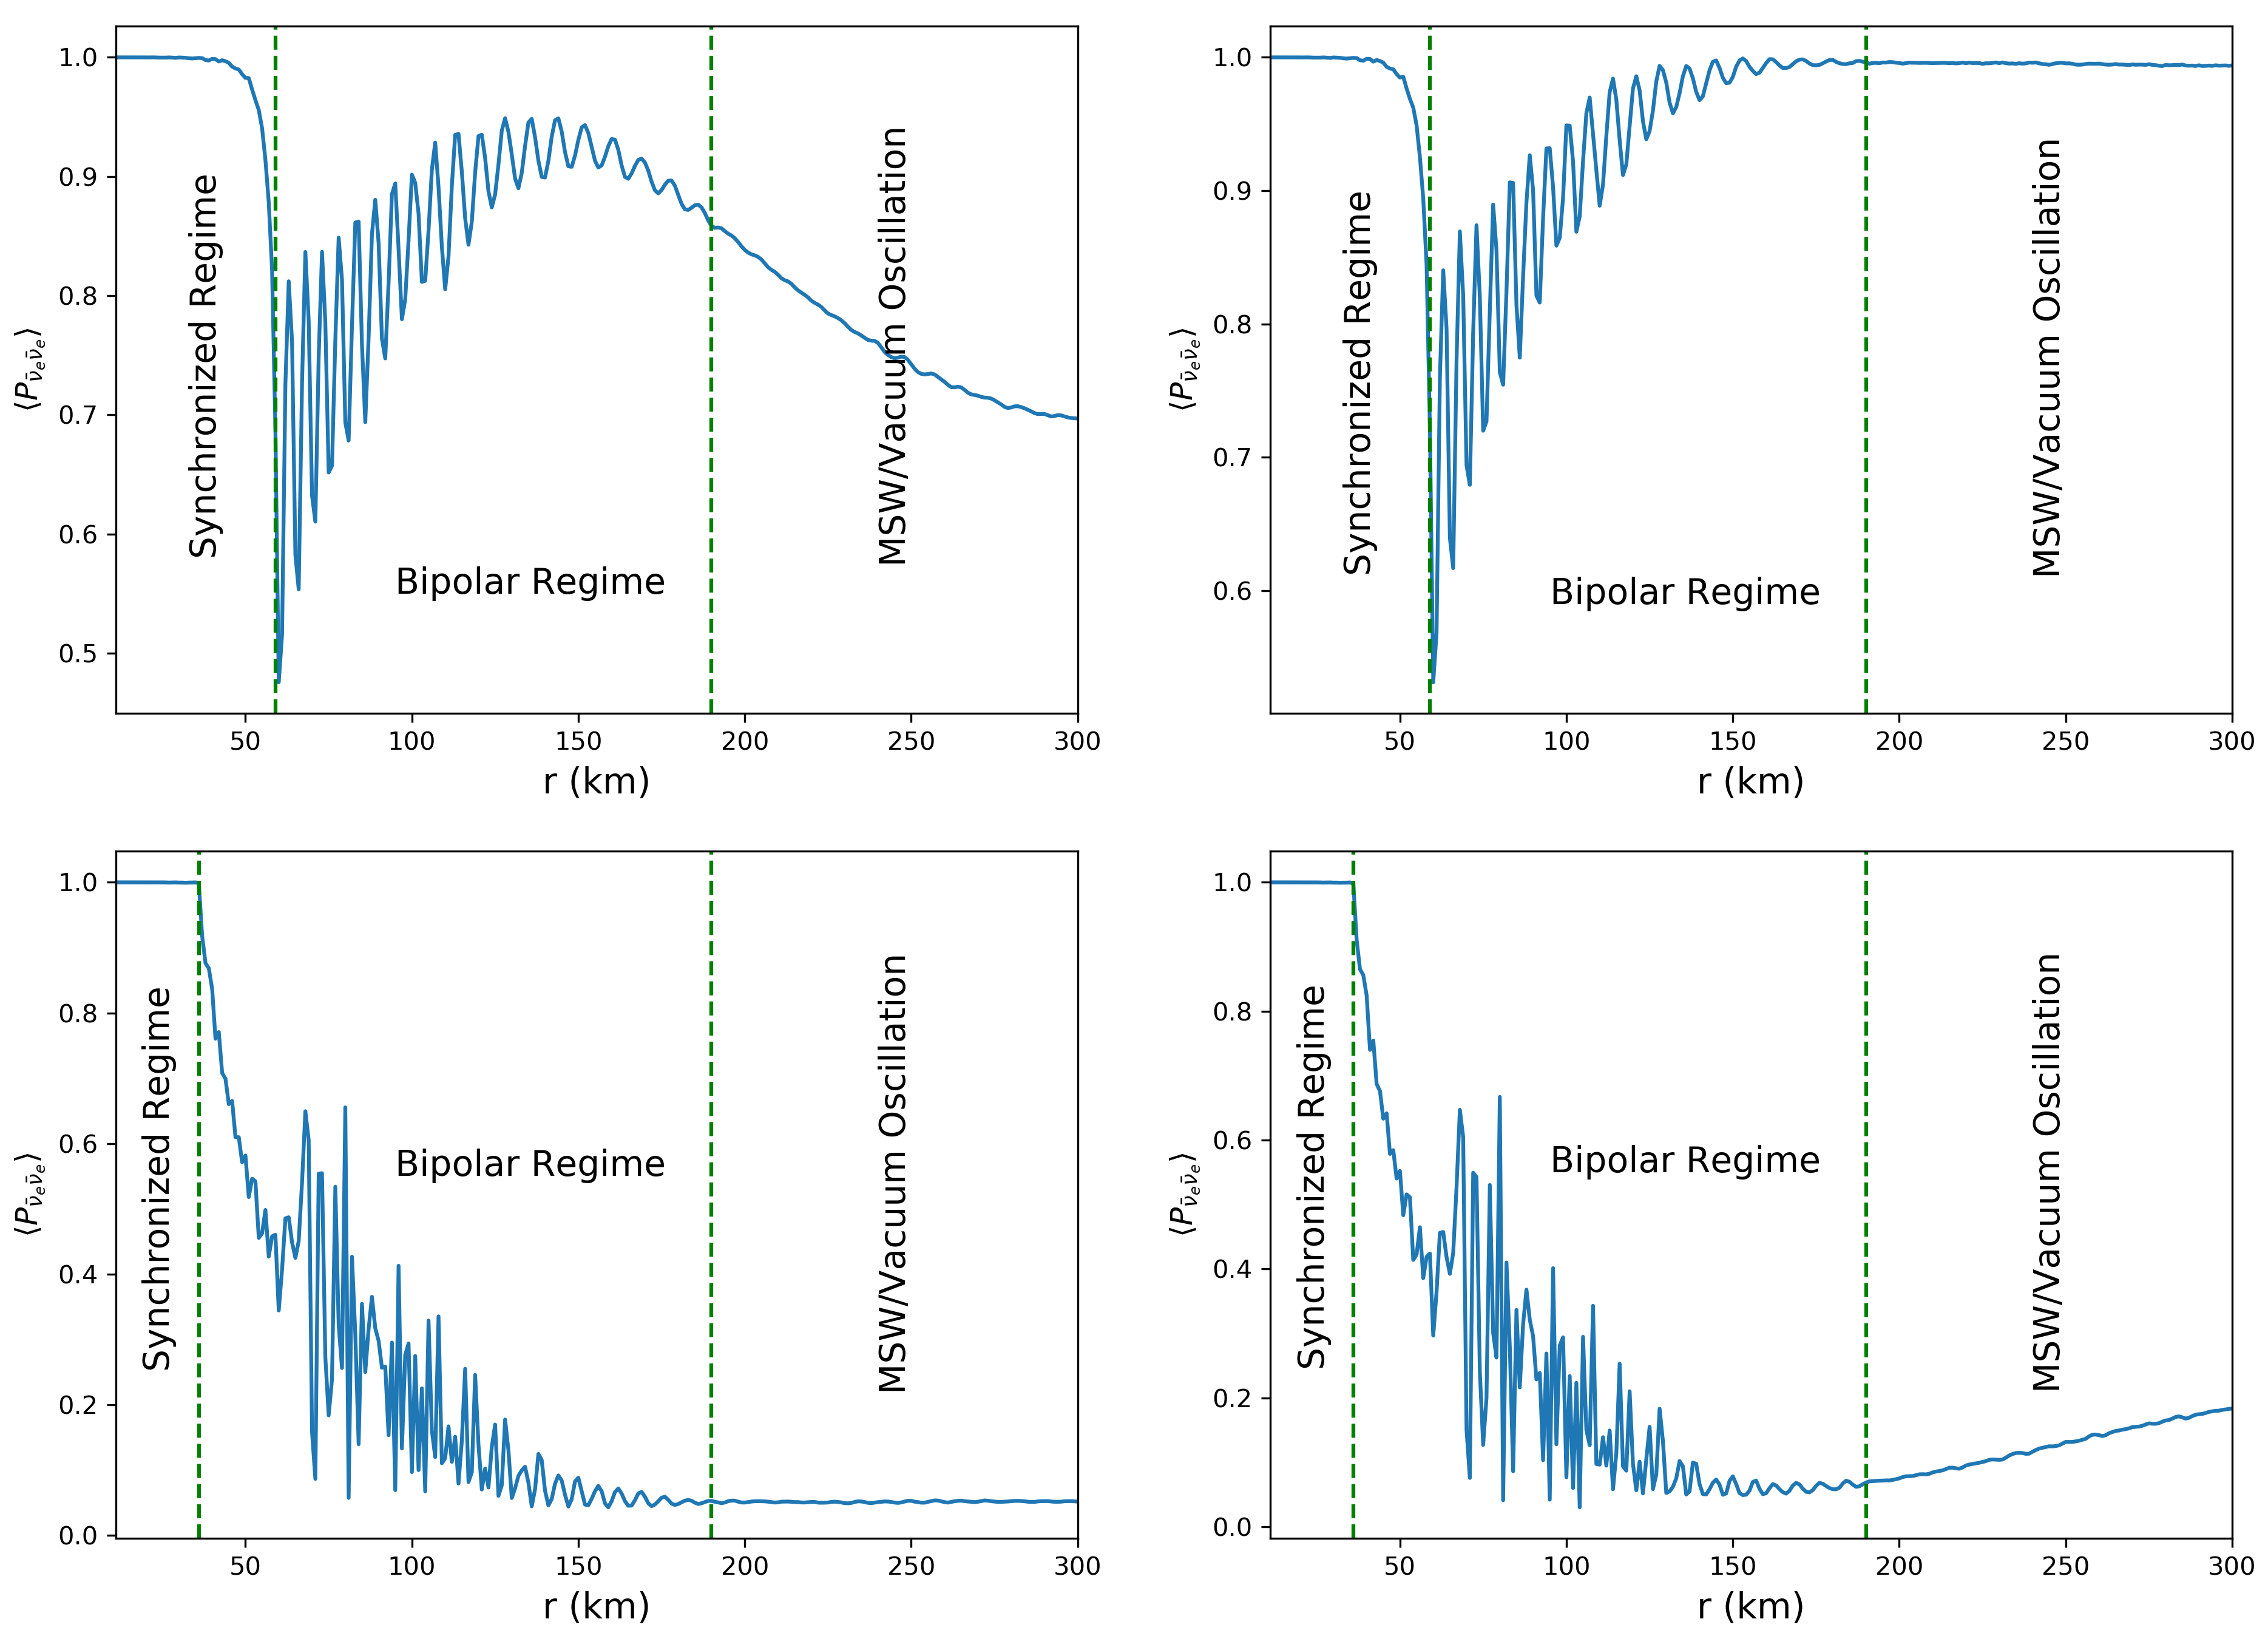
\includegraphics[width=\linewidth]{flavor_evo_std.png}
\caption{Plots of energy-averaged neutrino survival probability evolution in the core-collapsed supernova environment. The upper panels correspond to normal mass hierarchy, lower panels inverted mass hierarchy, left panel $\nu_e$, and right panels $\bar \nu_e$. Three oscillation regimes can be identified from the plots. Near the proto-neutron star is the synchronized regime, where collective oscillation are suppressed by either large matter density or neutrino density, and neutrinos experience $\nu$-enhanced MSW flavor transfromations. Far away from the star neutrino flux are negligible, and neutrinos undergo conventional vacuum/MSW oscillations. In between these two regions is the bipolar regime where neutrinos experience collective oscillation and spectral swap/split develop.} 
\label{fig:fe_std}
\end{center}
\end{figure}

\begin{figure}[t]
\begin{center}
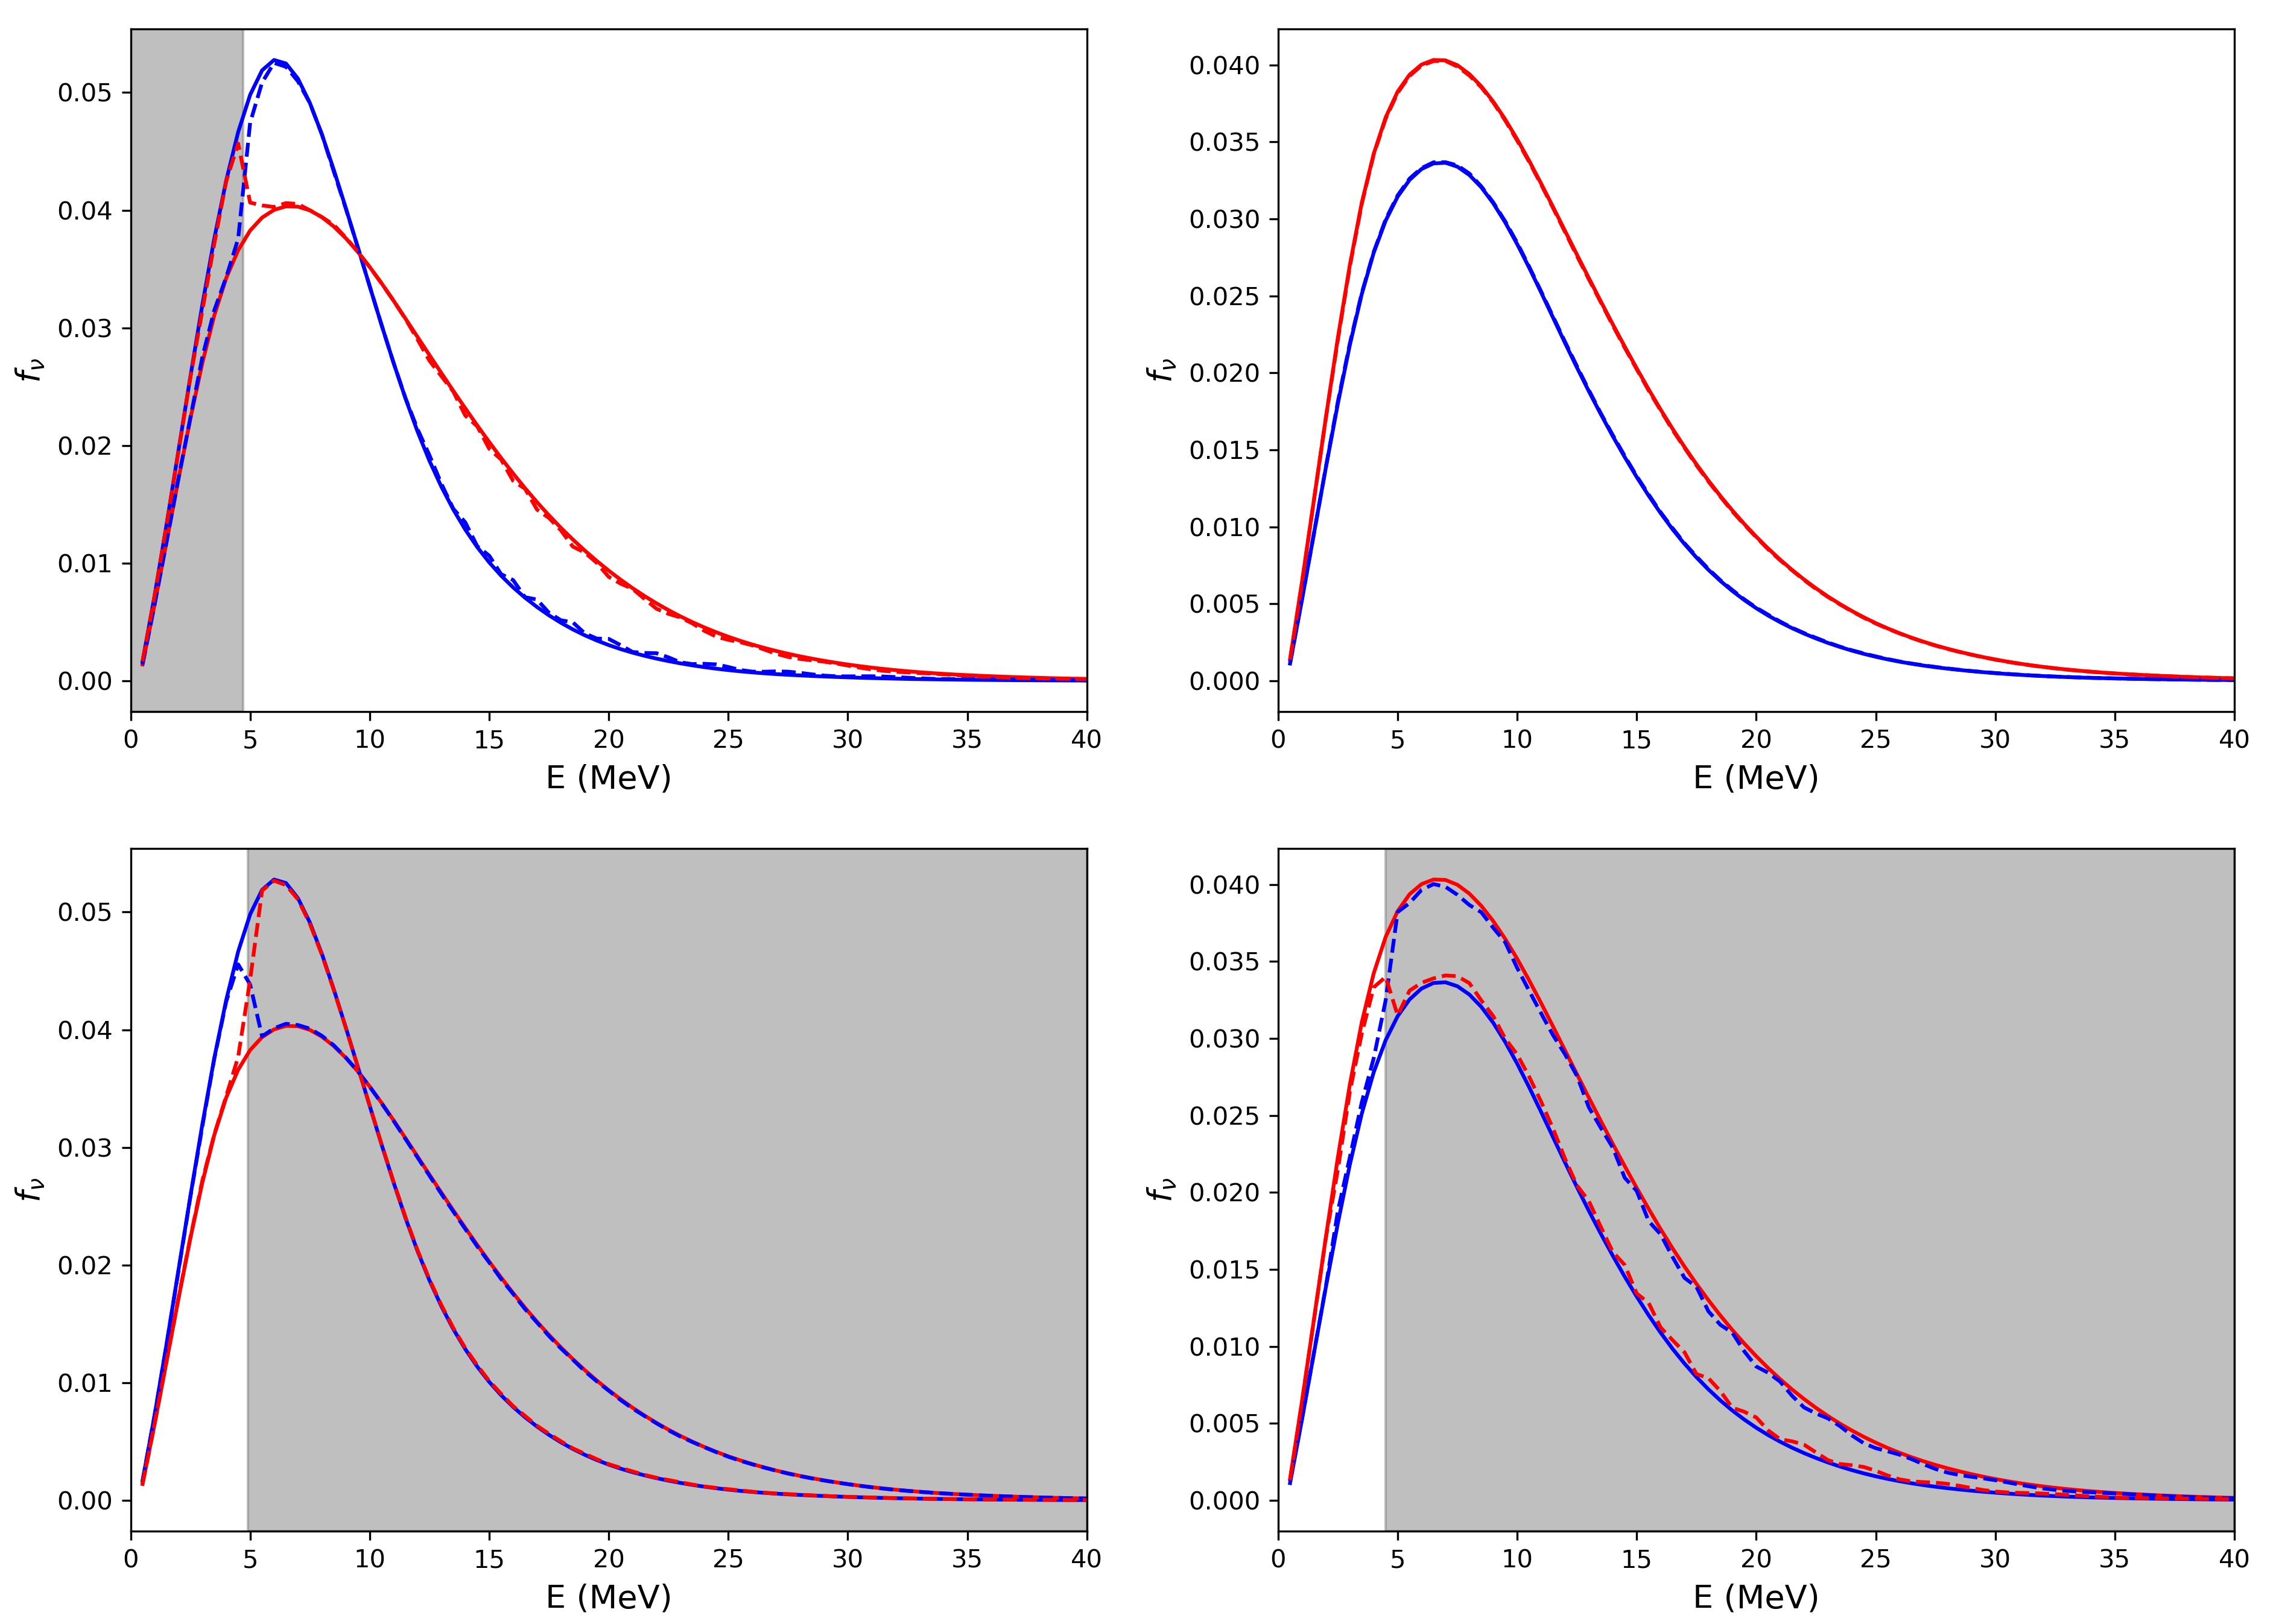
\includegraphics[width=\linewidth]{neutrino_spectra_std.png}
\caption{Plots of neutrino spectra before and after oscillation. The panels are ordered in the same way as figure 1. The solid lines represent spectra before oscillation, dashed lines after oscillation. The plots illustrate the characteristic feature of collective oscillation, the spectral split/swap phenomenon. The shaded regions in each plot correspond to the spectral swap regions, and the boundaries correspond to spectra split.}
\label{fig:spectra_std}
\end{center}
\end{figure}

\subsection{Oscillation with NSSI Modification}

Figure 3, 4 Key Points \& References:
\begin{itemize}
  \item Larger values of $g_3$ generally correspond to a delay of the onset time of bipolar collective oscillation, while larger values of $g_1$ correspond to an advance of that onset time, matching the basic predictions of references \cite{Dighe, Das}.
  \item The difference in energy-averaged final survival probability between different NSSI values allow us to make predictions for observables at the detector level. The final flux $F_e^f$ is given in terms of the initial fluxes $F_e$, $F_x$ and survival probability P as $F_e^f = P F_e + (1-P) F_x = P(F_e - F_x) + F_x$. During the late-time cooling phase, the flux hierarchy is $F_x > F_e/\bar F_e$ \cite{Nakasato}, therefore larger values of P correspond to a smaller final flux value. Looking at figure 3 and 4, we can predict that final flux in the fv-nssi scenario will be smaller than final flux in the fp-nssi and standard scenarios for anti-neutrinos in the IH case, and will be larger for neutrinos in the NH case. As the fluxes of different flavors become more and more degenerate during the cooling phase, this difference will decrease until it becomes zero when the fluxes are fully degenerate.
\end{itemize}

\begin{figure}[t]
\begin{center}
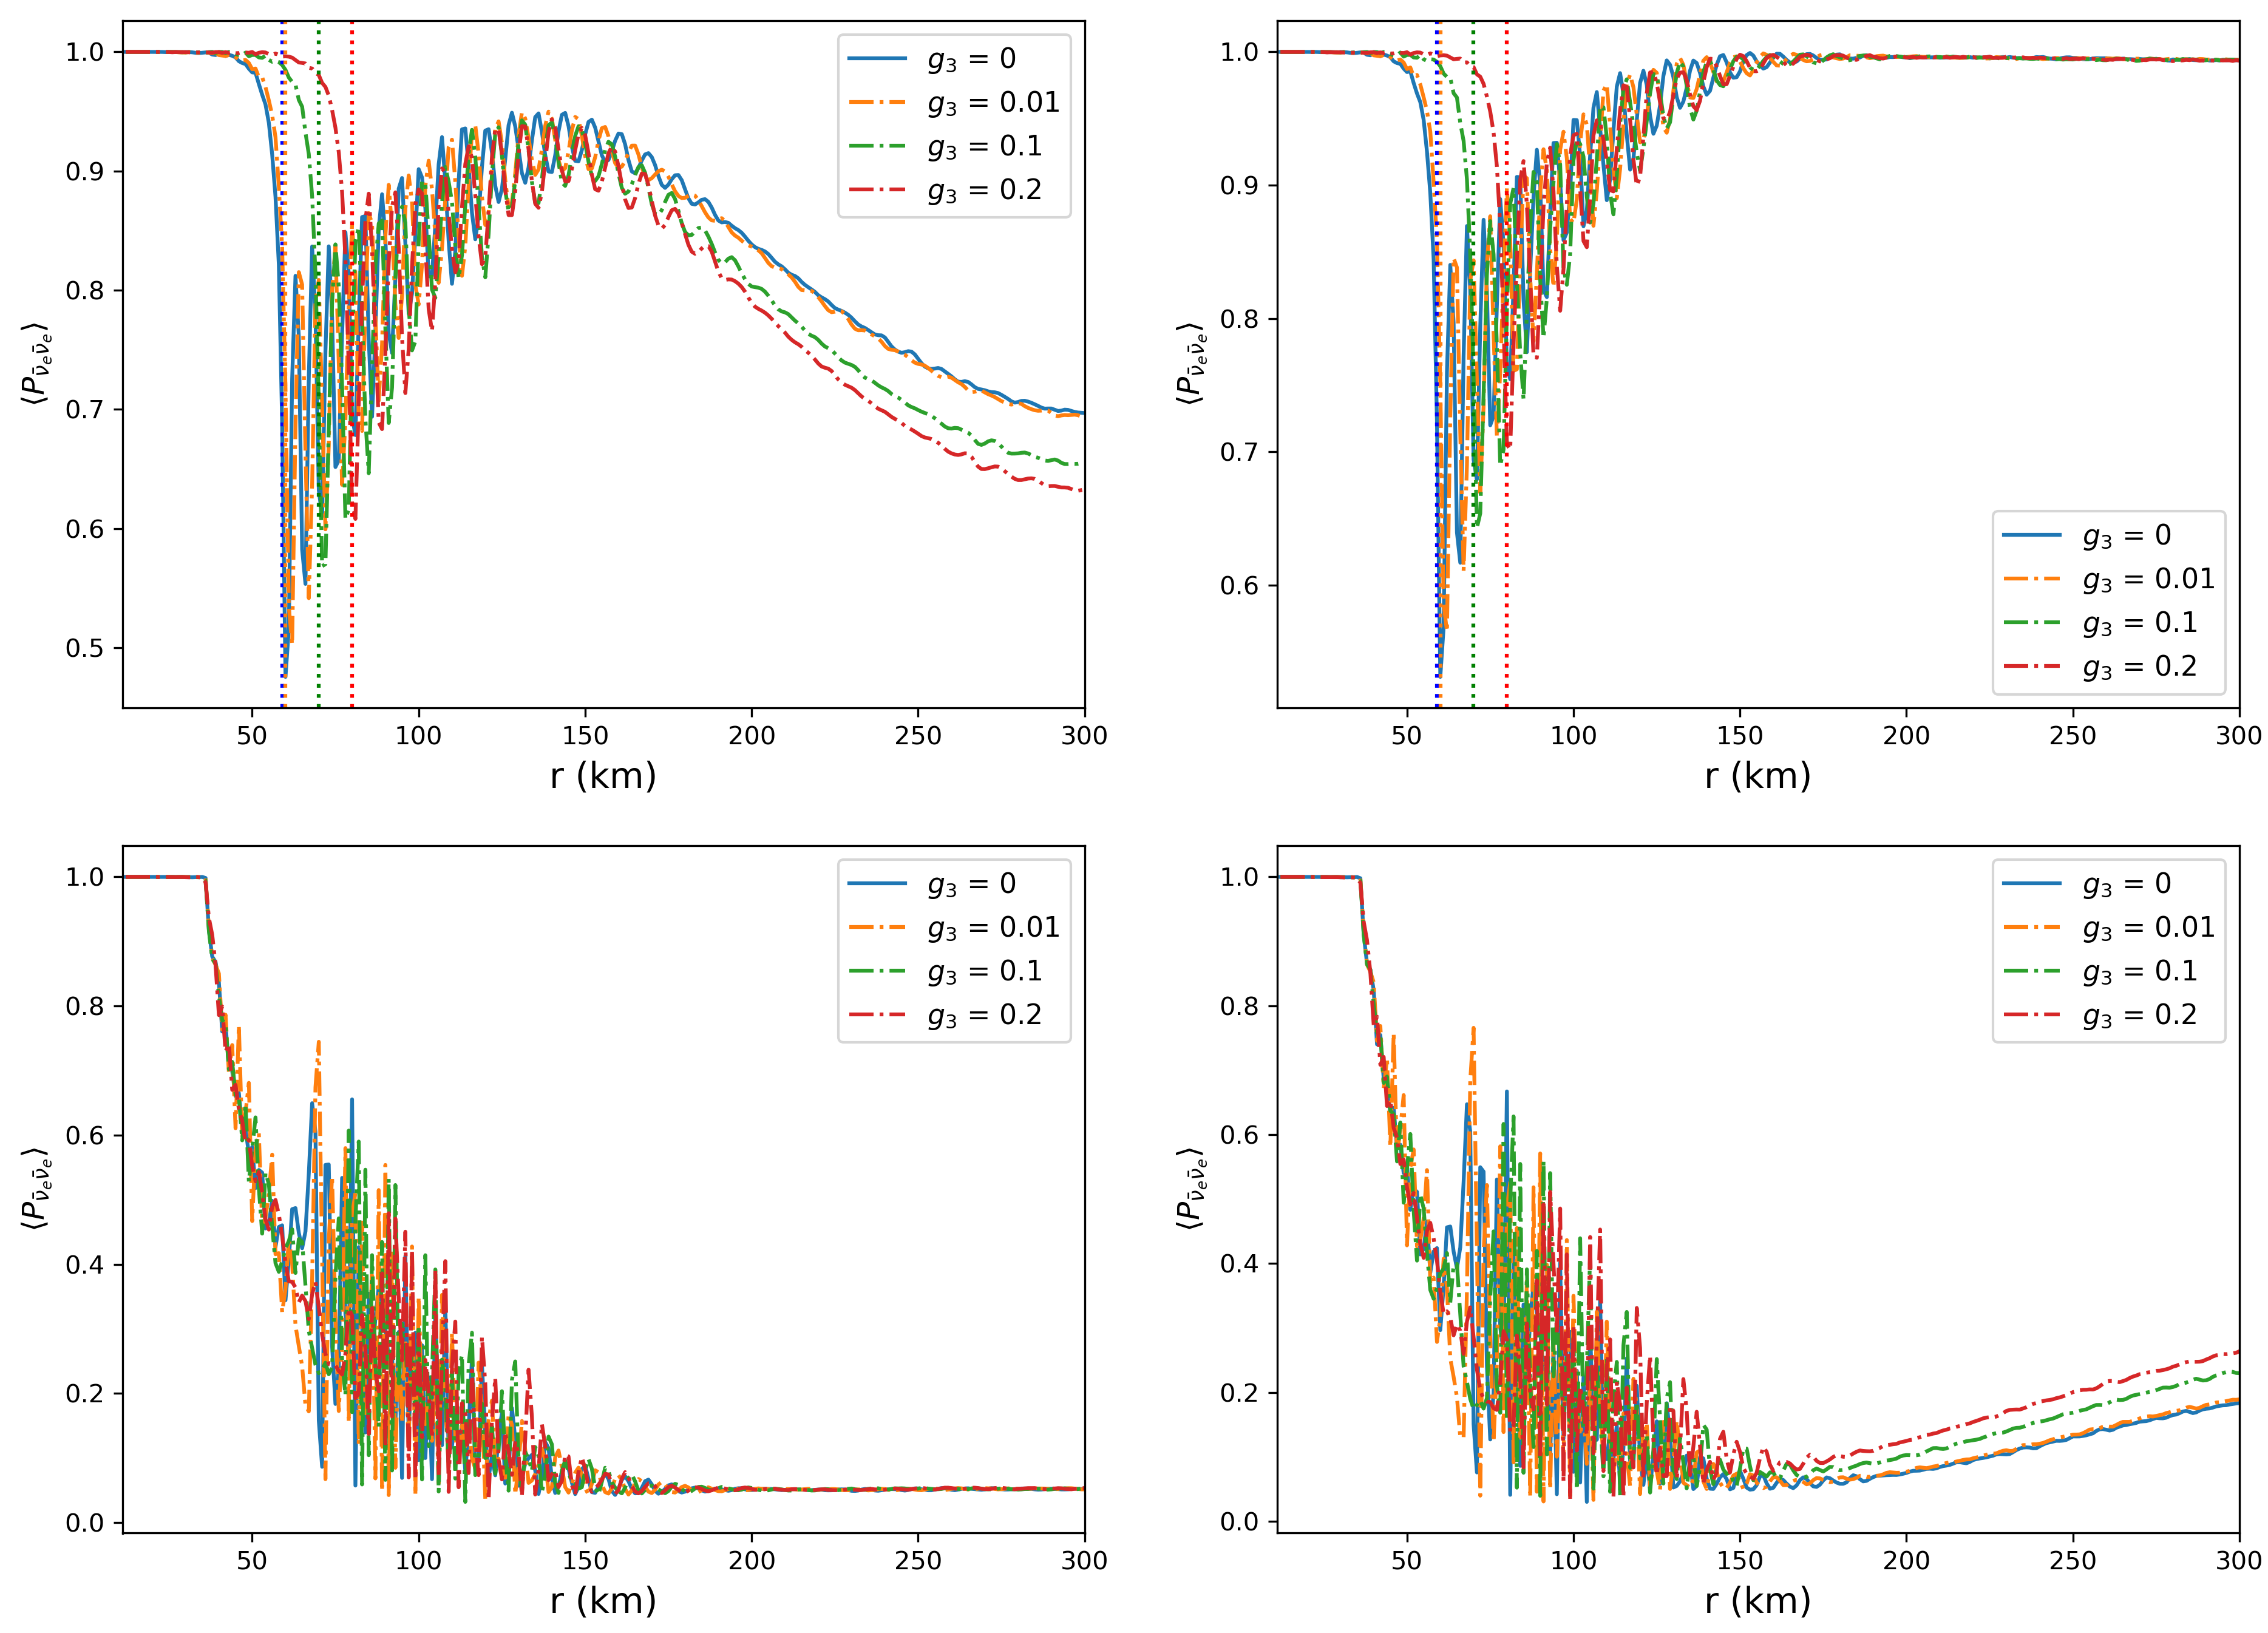
\includegraphics[width=\linewidth]{flavor_evo_fp.png}
\caption{Plots of energy-averaged flavor history plots with different values of fp-nssi parameter $g_3$, the fv-nssi parameter $g_1$ is set to zero for all cases. The panels are ordered as in figure 1. From the plots, larger values of $g_3$ correspond to a delay of the onset time of the bipolar regime in the NH case, as indicated by the vertical lines. The effect is less apparent in the IH case. Small differences in the final survival probability develops between different values of $g_3$ for $\nu_e$ in the NH case, and for $\bar \nu_e$ in the IH case.}
\label{fig:fe_fp}
\end{center}
\end{figure}

\begin{figure}[t]
\begin{center}
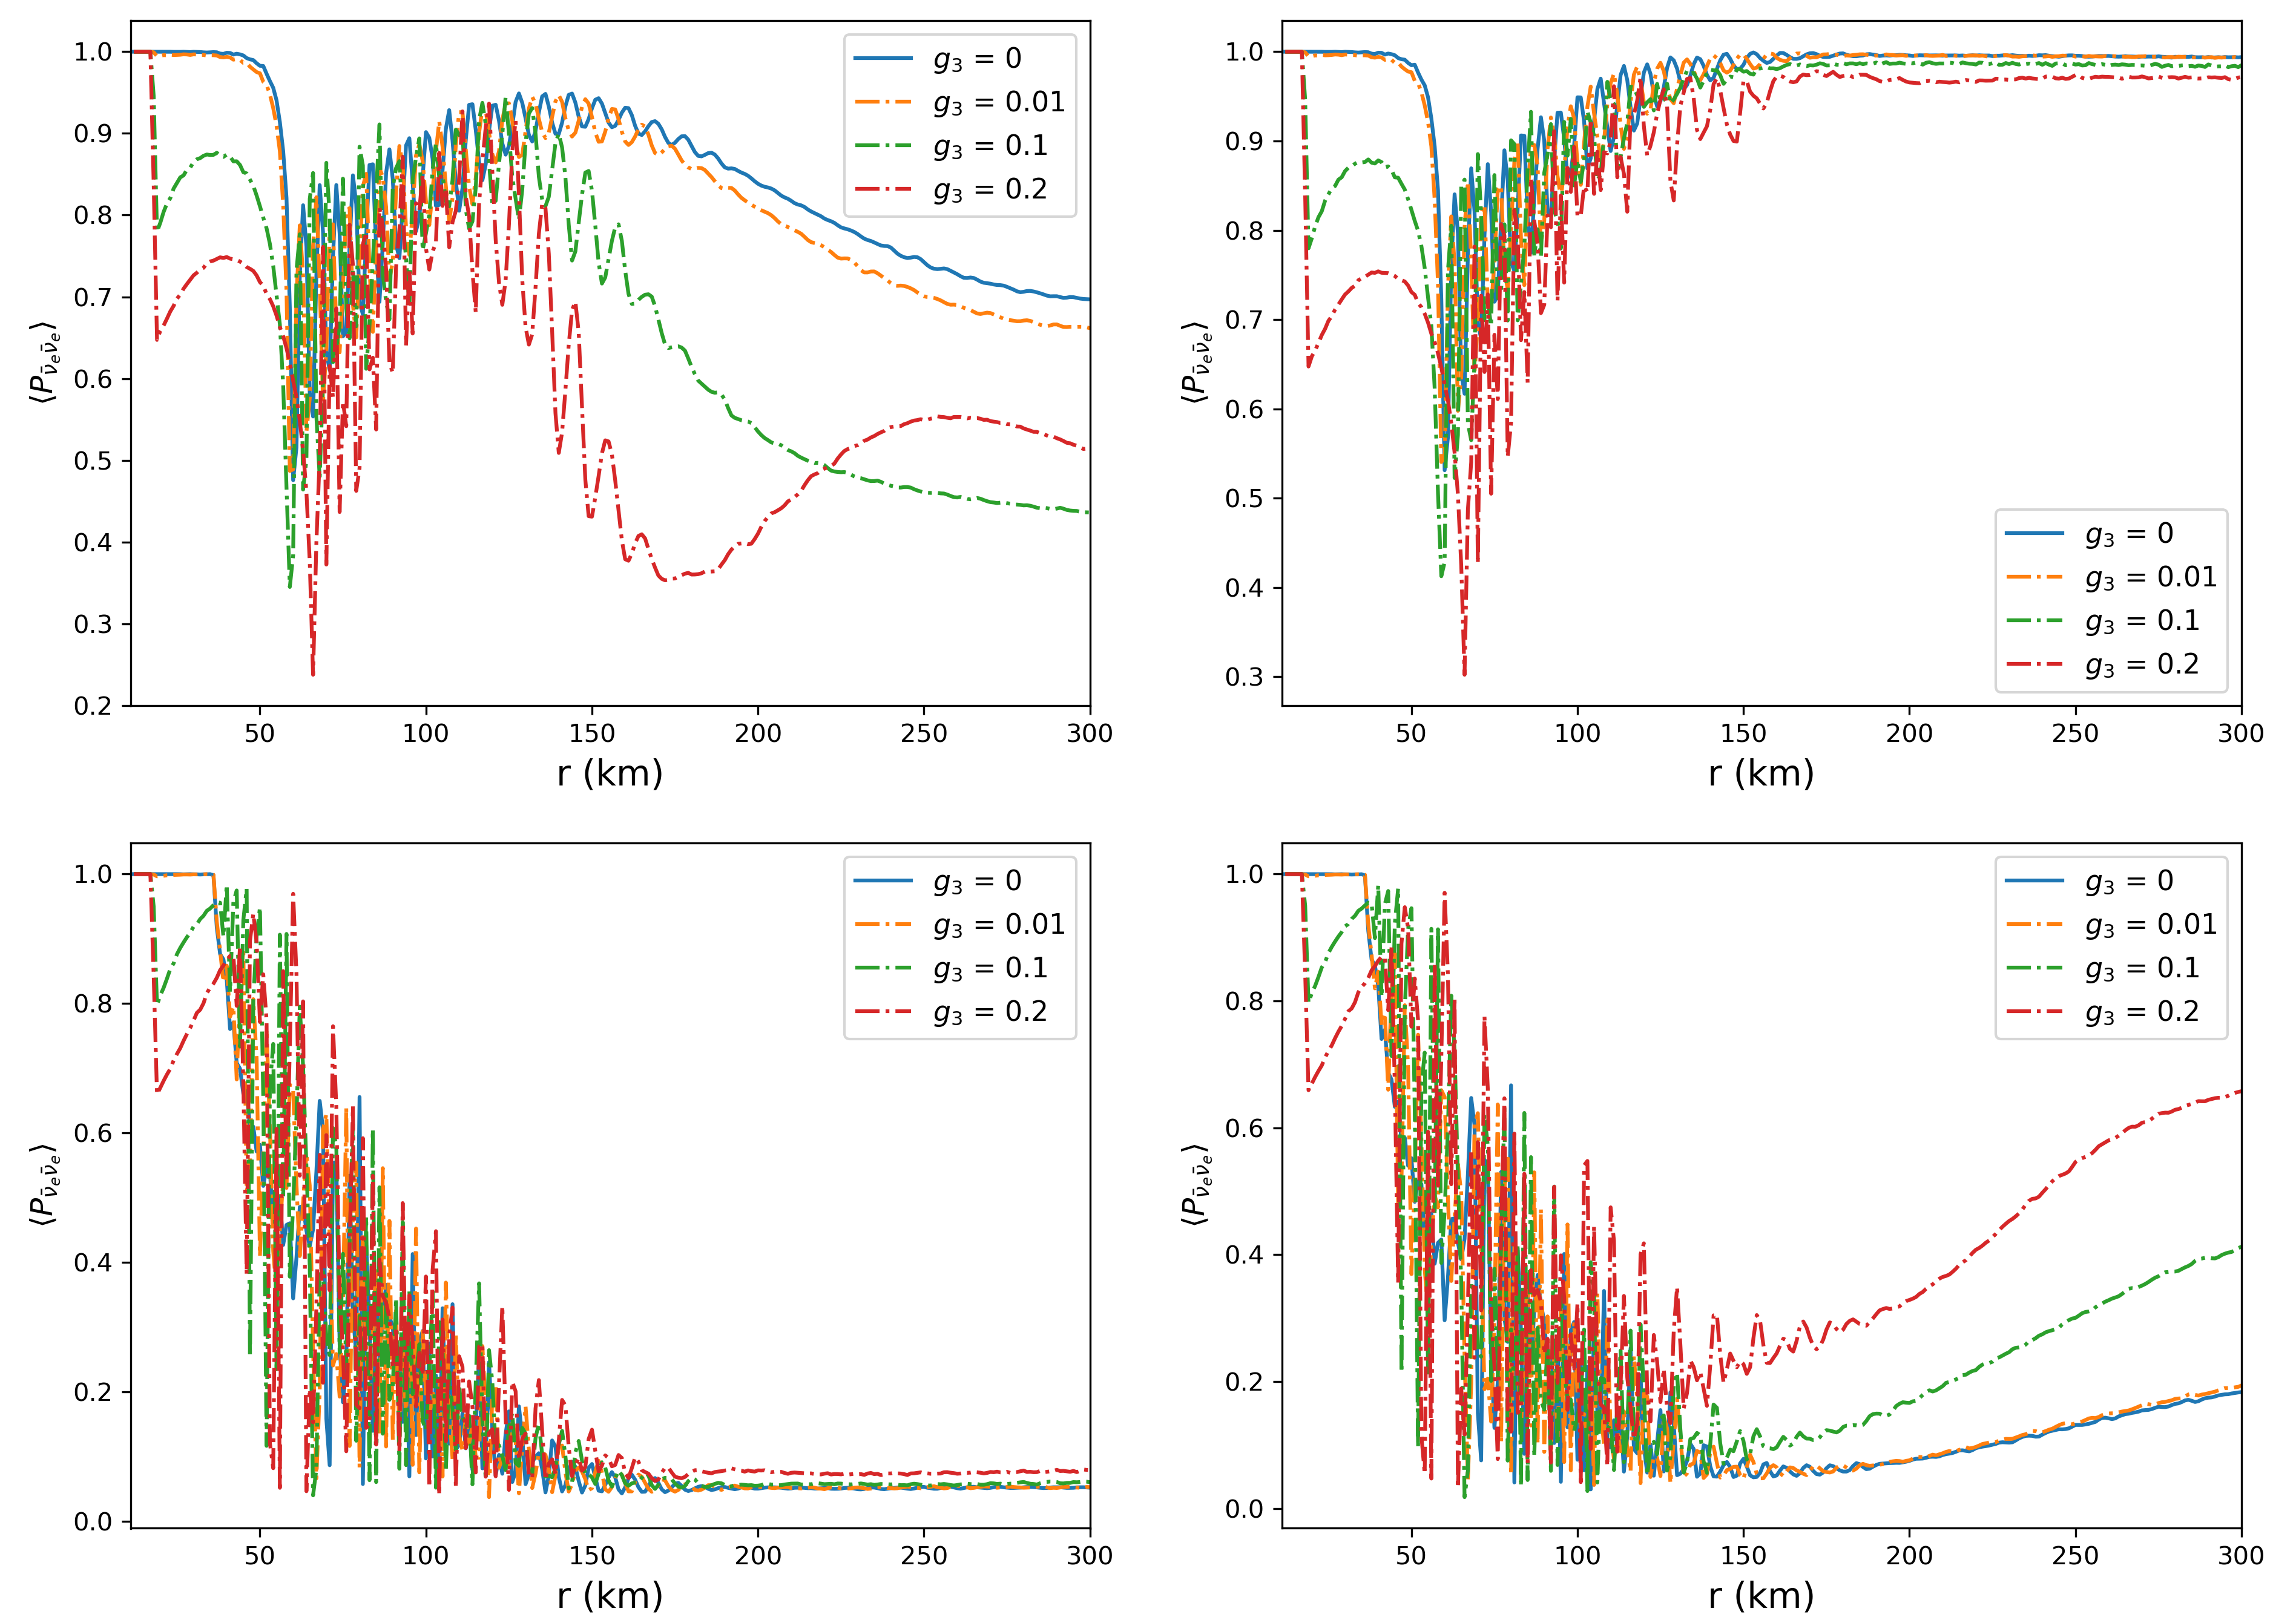
\includegraphics[width=\linewidth]{flavor_evo_fv.png}
\caption{Plots of energy-averaged flavor history plots with different values of fv-nssi parameter $g_1$, the fp-nssi parameter $g_3$ is set to zero for all cases. The panels are ordered as in figure 1. Here, larger values of $g_1$ correspond to an advance of the onset time of the bipolar regime in the NH case. Large differences can be observed in the final survival probability between different values of $g_3$ for $\nu_e$ in the NH case, and for $\bar \nu_e$ in the IH case.}
\label{fig:fe_fv}
\end{center}
\end{figure}

\section{Detector Data Simulation Results}

Figure 5 Key Points \& References:
\begin{itemize}
  \item Based on the numerical supernova simulation \cite{Nakasato}, neutrino flux and luminosity during the cooling phase are largely independent from supernova models. To further eliminate the dependence on distance of the supernova from the detector, we take the ratio between data from the IBD channel and the ES channel
  \item The difference in the detector data observable agrees with the basic prediction from figure 3, 4, expect for the ES case, where little statistics are available from a $H_2O$ detector like Hyper-K. Better ES statistics should be available from a liquid-Ar detector like DUNE and compliment the current data, allowing us to make a distinction in the NH case as well.
\end{itemize}

\begin{figure}[t]
\begin{center}
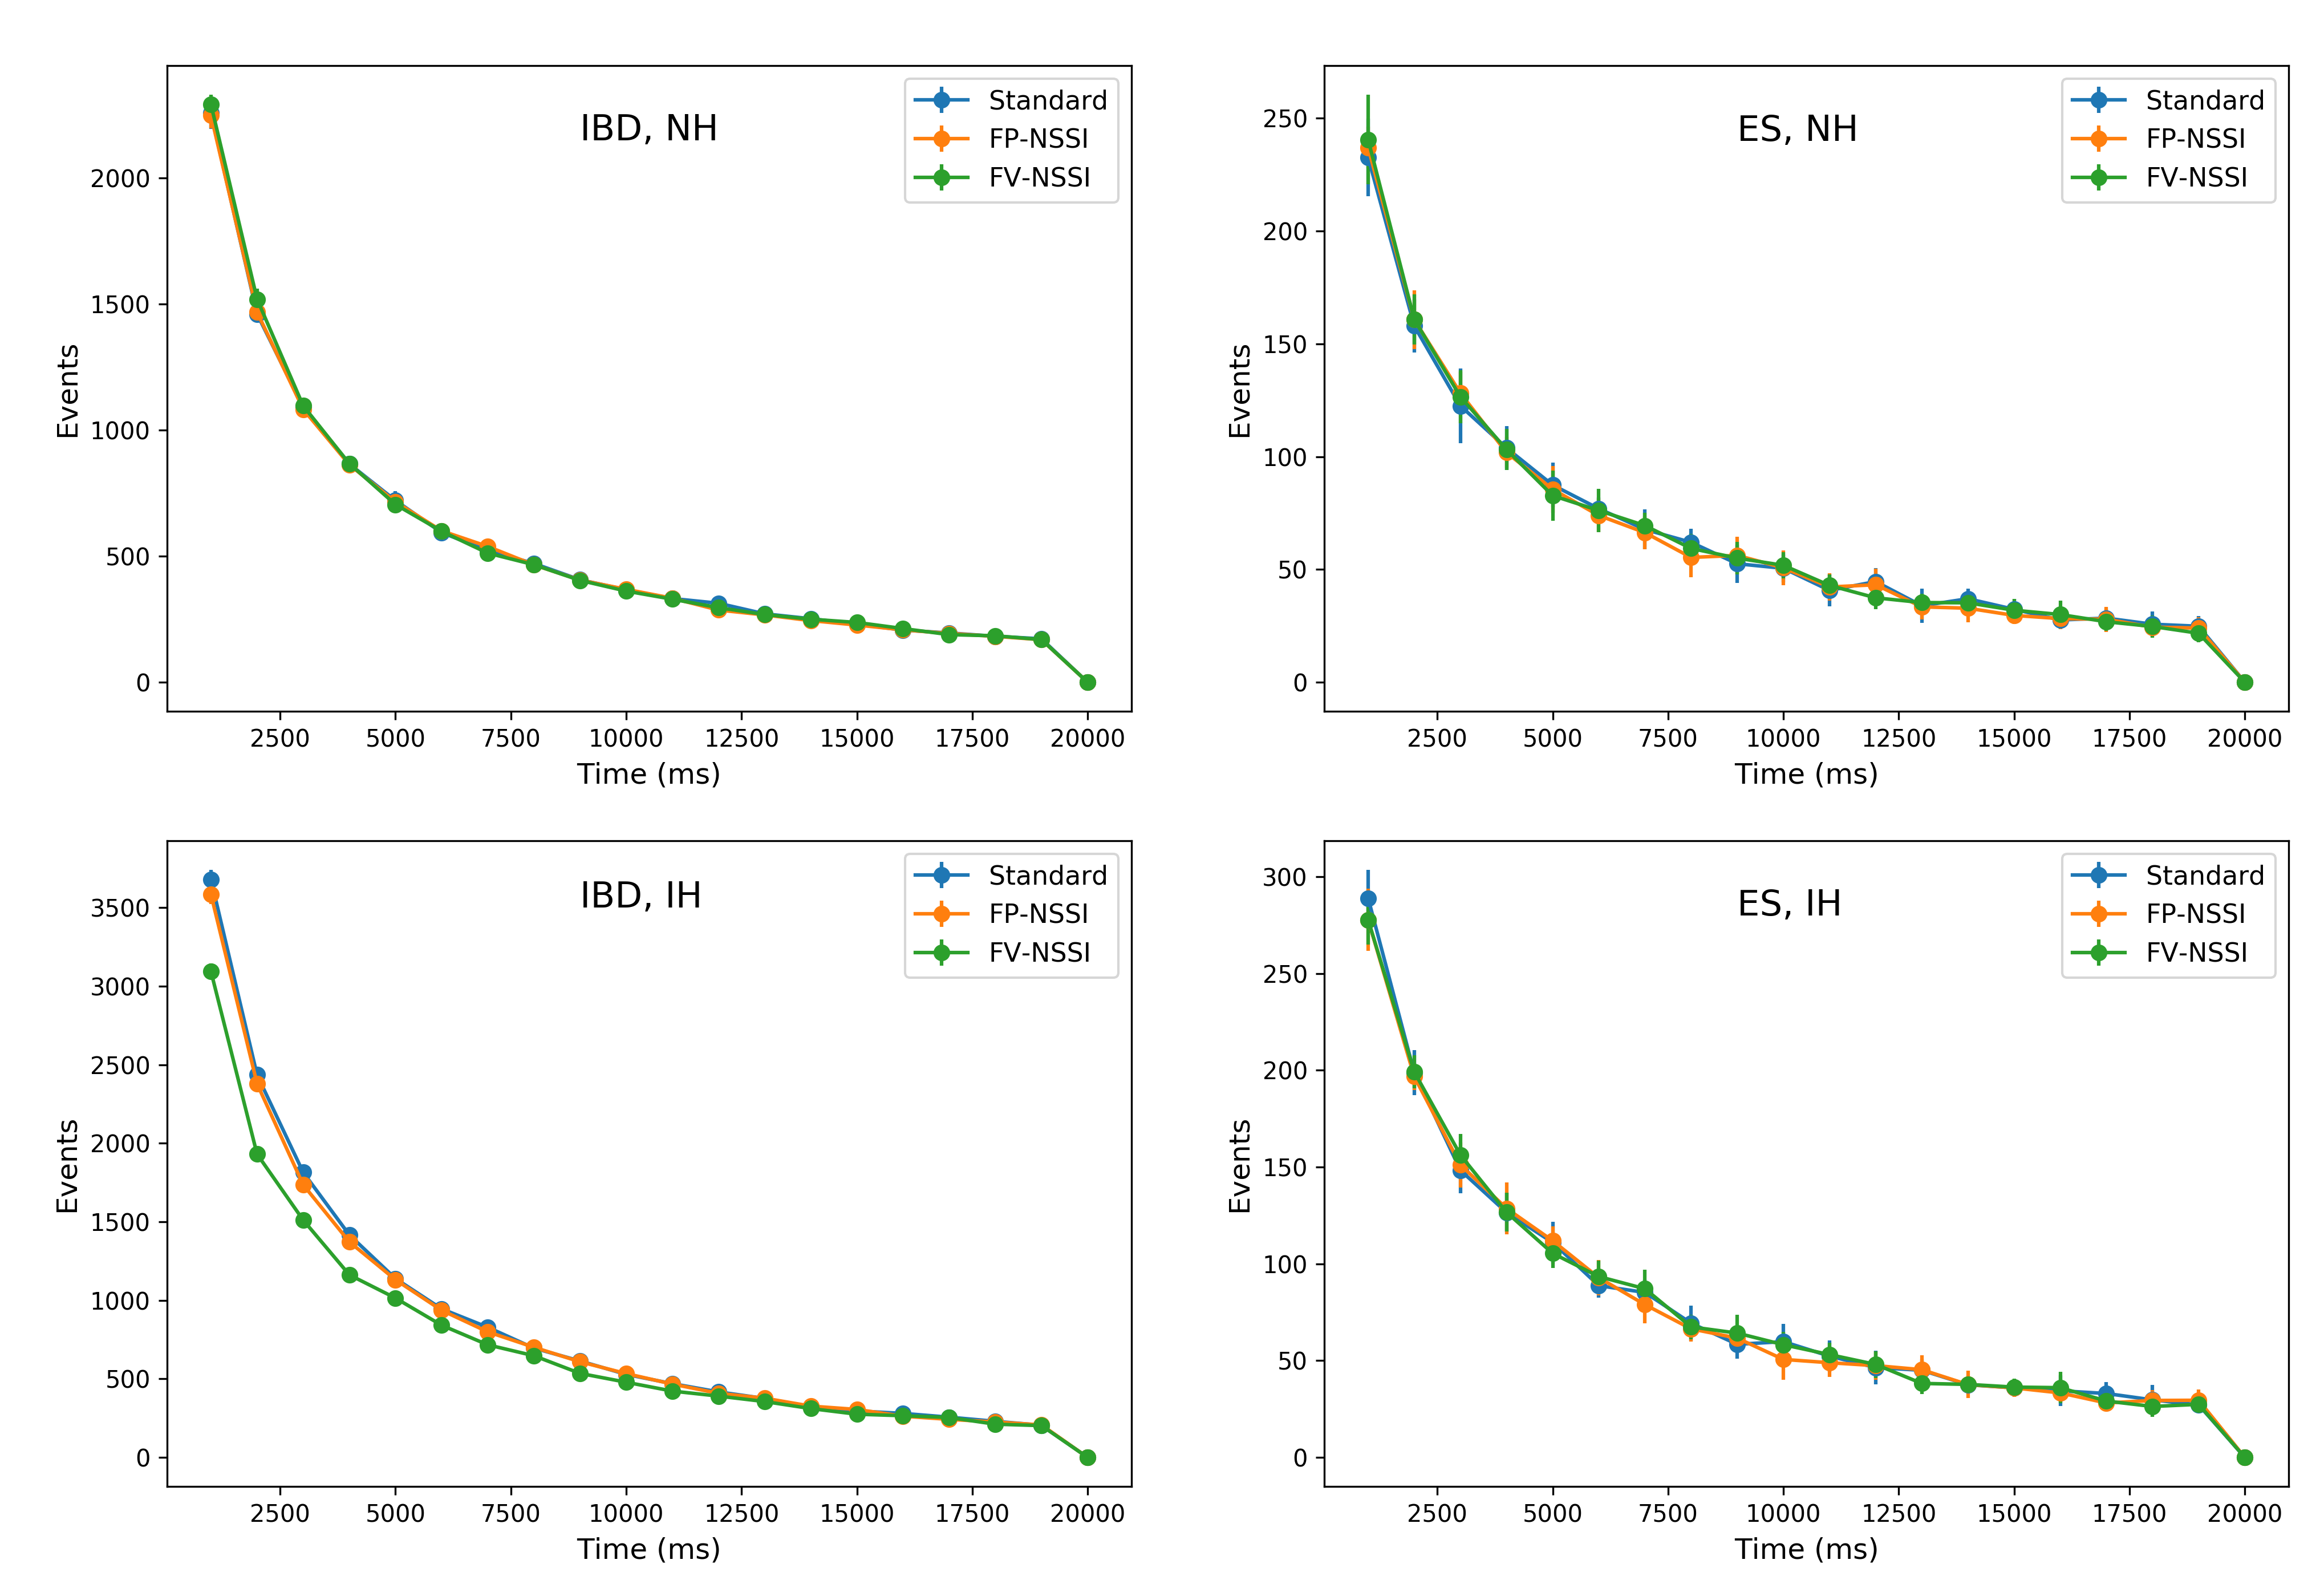
\includegraphics[width=\linewidth]{detector_data.png}
\caption{Plot of number of detected events over time. t = 0 is set to the time of the observed peak of the neutrino flux. The upper panels correspong to NH, lower panels IH, left panels the inverse beta decay channel, and the right panels the elastic scattering channel. Since the IBD channel correspond to $\bar \nu_e$ detection and ES channel mainly correspond to $\nu_e$ detection, as predicted by the flavor evolution plots in figure 3 and 4, we should expect to see significant difference between fv-nssi and fp-nssi/standard for IBD in the IH case, and for ES in the NH case, and the difference should decrease as neutrino fluxes become more degenerate over time. This is clearly the case for IBD channel. However, it is not observed in the ES channel, due to poor $\nu_e$ statistics from $H_2O$ detectors such as Hyper-K.}
\label{fig:detector_data}
\end{center}
\end{figure}

\begin{table}[t]
\caption{Ratio of total event detection during the late time regime in the elastic scattering channel over that in the inverse beta decay channel for both normal mass hierarchy and inverse mass hierarchy case. The ratio provide a largely model-independent signature for NSSI modifications. In this case, there is significant difference between fv-nssi and fp-nssi/standard in the IH case. With better ES channel statistics, such as from a liquid-Ar detector like DUNE,  we expect to see much smaller statistical variation in the ratios, and a difference in the NH case as well as predicted by the flavor history plots in figure 3, 4.}
\label{tab:evt_ratio}
\centering
\scalebox{1.1}{
\begin{tabular}{|c|c|c|c|}
\hline
\begin{tabular}[c]{@{}c@{}}Event \\ Ratio\end{tabular} & Standard & FP-NSSI & FV-NSSI \\ \hline
NH & 11.99$\pm$0.40 & 11.97$\pm$0.26 & 11.96$\pm$0.29 \\ 
IH & 9.30$\pm$0.11 & 9.34$\pm$0.21 & 10.72$\pm$0.25 \\ \hline
\end{tabular}}
\end{table}

\begin{thebibliography}{9}
\bibitem{Duan1} 
Duan, H., Fuller, G. M., Carlson, J., \& Qian, Y. Z. (2006). Simulation of coherent nonlinear neutrino flavor transformation in the supernova environment: Correlated neutrino trajectories. Physical Review D, 74(10), 105014.

\bibitem{Duan2} 
Duan, H., Fuller, G. M., \& Carlson, J. (2008). Simulating nonlinear neutrino flavor evolution. Computational Science \& Discovery, 1(1), 015007.

\bibitem{Duan3}
Duan, H., Fuller, G. M., \& Qian, Y. Z. (2006). Collective neutrino flavor transformation in supernovae. Physical Review D, 74(12), 123004.

\bibitem{Blennow} 
Blennow, M., Mirizzi, A., \& Serpico, P. D. (2008). Nonstandard neutrino-neutrino refractive effects in dense neutrino gases. Physical Review D, 78(11), 113004.

\bibitem{Nakasato} 
Nakazato, K. I., Sumiyoshi, K., Suzuki, H., Totani, T., Umeda, H., \& Yamada, S. (2013). Supernova neutrino light curves and spectra for various progenitor stars: from core collapse to proto-neutron star cooling. The Astrophysical Journal Supplement Series, 205(1), 2.

\bibitem{HK} 
Abe, K., Abe, K., Aihara, H., Aimi, A., Akutsu, R., Andreopoulos, C., ... \& Aushev, V. (2018). Hyper-Kamiokande design report. arXiv preprint arXiv:1805.04163.

\bibitem{Chakraborty} 
Chakraborty, S., Fischer, T., Mirizzi, A., Saviano, N., \& Tomas, R. (2011). Analysis of matter suppression in collective neutrino oscillations during the supernova accretion phase. Physical Review D, 84(2), 025002.

\bibitem{Dighe} 
Dighe, A., \& Sen, M. (2018). Nonstandard neutrino self-interactions in a supernova and fast flavor conversions. Physical Review D, 97(4), 043011.

\bibitem{Das} 
Das, A., Dighe, A., \& Sen, M. (2017). New effects of non-standard self-interactions of neutrinos in a supernova. Journal of Cosmology and Astroparticle Physics, 2017(05), 051.

\end{thebibliography}

\end{document}  